\documentclass[tikz,border=4pt]{standalone}
\usepackage{mathptmx}
\usetikzlibrary{positioning,arrows.meta,fit,calc}
\begin{document}
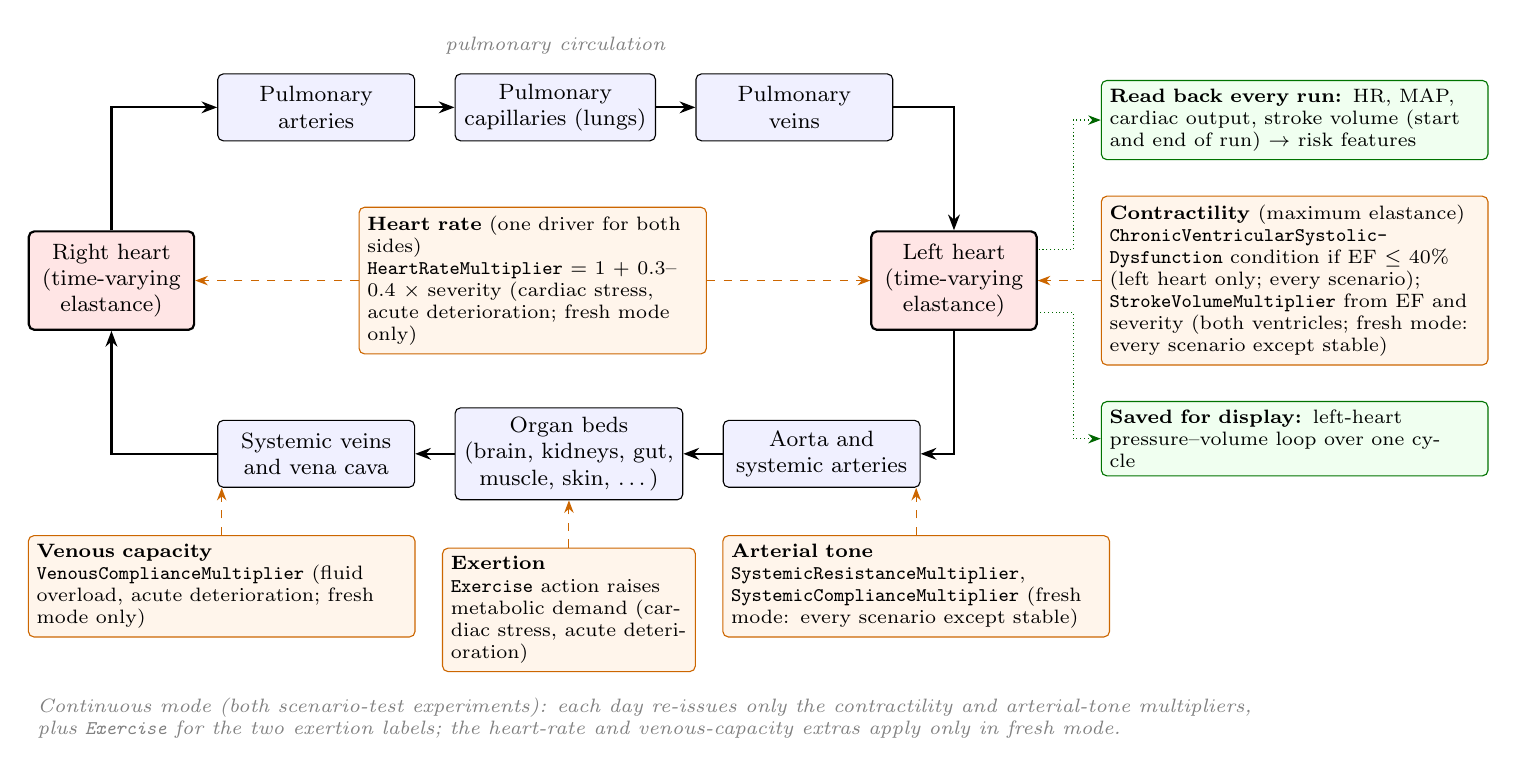
\begin{tikzpicture}[font=\footnotesize,
  comp/.style={draw, rounded corners=2pt, fill=blue!6, minimum width=2.5cm, minimum height=0.85cm, align=center},
  heart/.style={draw, rounded corners=2pt, fill=red!10, minimum width=2.1cm, minimum height=1.25cm, align=center, thick},
  mod/.style={draw=orange!80!black, fill=orange!8, rounded corners=2pt, align=left, font=\scriptsize, text width=4.7cm, inner sep=3pt},
  outp/.style={draw=green!45!black, fill=green!6, rounded corners=2pt, align=left, font=\scriptsize, text width=4.7cm, inner sep=3pt},
  flow/.style={-{Stealth[length=2mm]}, thick},
  act/.style={-{Stealth[length=1.6mm]}, dashed, orange!80!black},
  meas/.style={{Stealth[length=1.6mm]}-, densely dotted, green!40!black}]
% pulmonary loop (top)
\node[comp] (pa) at (0,2.2) {Pulmonary\\arteries};
\node[comp, right=0.5cm of pa] (lung) {Pulmonary\\capillaries (lungs)};
\node[comp, right=0.5cm of lung] (pv) {Pulmonary\\veins};
% hearts
\node[heart] (rh) at (-2.6,0) {Right heart\\(time-varying\\elastance)};
\node[heart] (lh) at (8.1,0) {Left heart\\(time-varying\\elastance)};
% systemic loop (bottom)
\node[comp] (sv) at (0,-2.2) {Systemic veins\\and vena cava};
\node[comp, right=0.5cm of sv] (org) {Organ beds\\(brain, kidneys, gut,\\muscle, skin, \ldots)};
\node[comp, right=0.5cm of org] (ao) {Aorta and\\systemic arteries};
% blood flow
\draw[flow] (rh.north) |- (pa.west);
\draw[flow] (pa) -- (lung);
\draw[flow] (lung) -- (pv);
\draw[flow] (pv.east) -| (lh.north);
\draw[flow] (lh.south) |- (ao.east);
\draw[flow] (ao) -- (org);
\draw[flow] (org) -- (sv);
\draw[flow] (sv.west) -| (rh.south);
\node[font=\scriptsize\itshape, gray, above=0.12cm of lung] {pulmonary circulation};
\node[font=\scriptsize\itshape, gray, below=0.12cm of org.south, yshift=-1.35cm] {};
% modifiers set by the pipeline (orange)
\node[mod, right=0.8cm of lh] (m1) {\textbf{Contractility} (maximum elastance)\\
  \texttt{ChronicVentricularSystolic-} \texttt{Dysfunction} condition if EF $\le$ 40\% (left heart only; every scenario);\\
  \texttt{StrokeVolumeMultiplier} from EF and severity (both ventricles; fresh mode: every scenario except stable)};
\node[mod, text width=4.2cm] (m2) at (2.75,0) {\textbf{Heart rate} (one driver for both sides)\\
  \texttt{HeartRateMultiplier} = 1 + 0.3--0.4 $\times$ severity (cardiac stress, acute deterioration; fresh mode only)};
\node[mod, below=0.6cm of ao, xshift=1.2cm] (m3) {\textbf{Arterial tone}\\
  \texttt{SystemicResistanceMultiplier}, \texttt{SystemicComplianceMultiplier} (fresh mode: every scenario except stable)};
\node[mod, below=0.6cm of sv, xshift=-1.2cm] (m4) {\textbf{Venous capacity}\\
  \texttt{VenousComplianceMultiplier} (fluid overload, acute deterioration; fresh mode only)};
\node[mod, below=0.6cm of org, text width=3.0cm] (m5) {\textbf{Exertion}\\
  \texttt{Exercise} action raises metabolic demand (cardiac stress, acute deterioration)};
\draw[act] (m1.west) -- (lh.east);
\draw[act] (m2.east) -- (lh.west);
\draw[act] (m2.west) -- (rh.east);
\draw[act] (m3.north) -- (ao.south -| m3.north);
\draw[act] (m4.north) -- (sv.south -| m4.north);
\draw[act] (m5.north) -- (org.south);
% outputs read by the pipeline (green)
\node[outp, above=0.45cm of m1] (o1) {\textbf{Read back every run:} HR, MAP, cardiac output, stroke volume (start and end of run) $\rightarrow$ risk features};
\node[outp, below=0.45cm of m1] (o2) {\textbf{Saved for display:} left-heart pressure--volume loop over one cycle};
\draw[meas] (o1.west) -- ++(-0.35,0) |- ($(lh.east)+(0,0.4)$);
\draw[meas] (o2.west) -- ++(-0.35,0) |- ($(lh.east)+(0,-0.4)$);
\node[font=\scriptsize\itshape, gray, align=left, anchor=north west] at ($(m4.west |- m5.south)+(0,-0.2)$) {Continuous mode (both scenario-test experiments): each day re-issues only the contractility and arterial-tone multipliers,\\plus \texttt{Exercise} for the two exertion labels; the heart-rate and venous-capacity extras apply only in fresh mode.};
\end{tikzpicture}
\end{document}
